\section{Value Proposition and Buisness Model}
The hypothethis is made that the customers and the users of this product are different. Indeed the people buying the device will be the family of the elder(s). While the elders will be the end users. Therefore the needs of the buyers and of the users are different. They will be both be using the device but through two different interfaces.

The

\subsection{Value Proposition}
As the customers and the users are not the same people we made two value proposition canvases.
The value propostion canvas for the elderly can be seen in figure \ref{fig:value proposition}.

\begin{figure}[!htb]
    \centering
    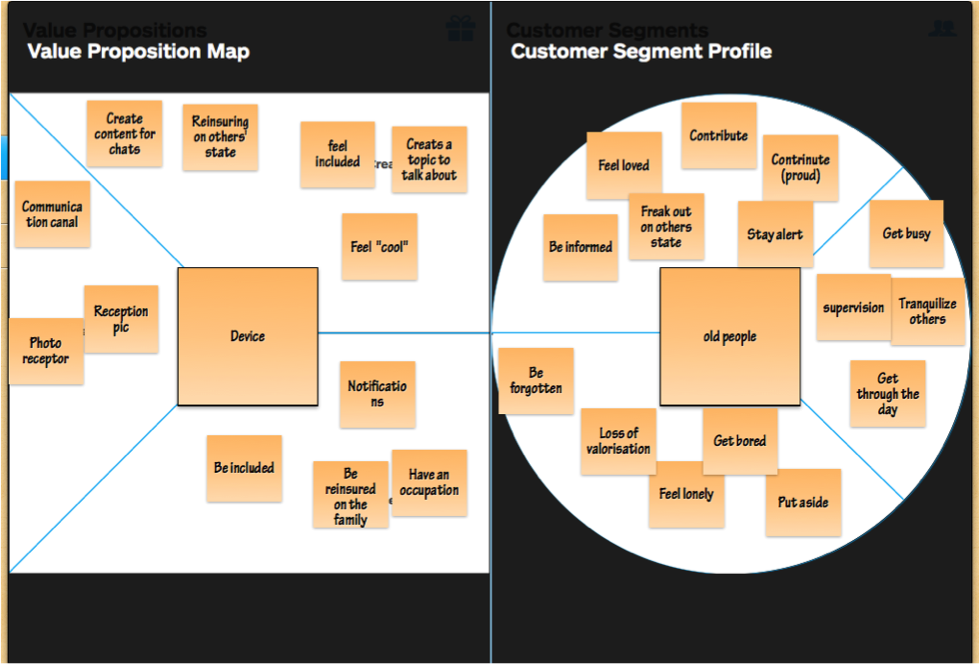
\includegraphics[width=0.9\textwidth,keepaspectratio]{chap/marketFig/elderly_value_prop_canvas.png}
    \caption{Buisness model canvas}
    \label{fig:elders value proposition}
\end{figure}

\subsection{Buisness model}

The buisness model canvas is shown in the figure \ref{fig:buisness model}.

\begin{figure}[!htb]
    \centering
    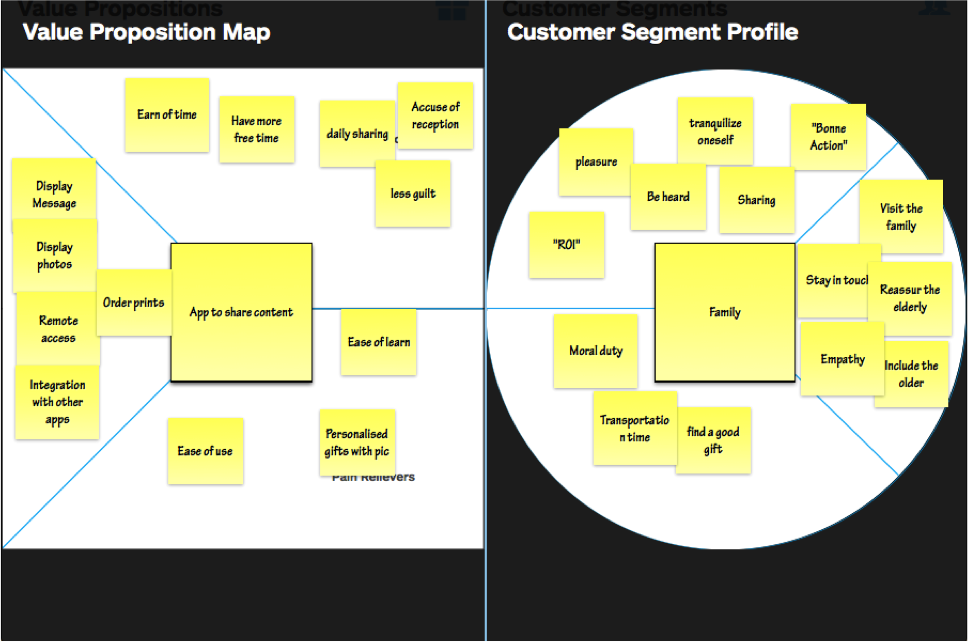
\includegraphics[width=0.9\textwidth,keepaspectratio]{chap/marketFig/family_value_prop_canvas.png}
    \caption{Buisness model canvas}
    \label{fig:buisness model}
\end{figure}

\subsection{User tests}
